\chapter{Results and Discussion}
\section{Recorded Prototype Results}
Table~\ref{tab:counts} summarizes the output sizes recorded in the experiment logs and progress presentation. Counts describe generated samples, not accuracy, measured surface coverage, or a fair ranking between methods.
\begin{table}[htbp]
\centering\small
\begin{tabular}{lrrr}
\toprule
Prototype & Object points & Background & Combined\\
\midrule
Bottle & 57,600 & --- & 57,600\\
Watch & 64,511 & 90,000 & 154,511\\
AC remote & 80,258 & 90,000 & 170,258\\
\bottomrule
\end{tabular}
\caption{Recorded point counts for the three coarse prototypes.}\label{tab:counts}
\end{table}

\subsection{Bottle Result}
The bottle experiment generated a 57,600-point colored cloud with estimated normals. The selected segmentation confidences were 0.765 for the left image, 0.683 for the right image, and 0.548 for the center image; the center detection used the vase class. These are model detection scores, not geometric confidence estimates.

Figure~\ref{fig:bottle} reproduces the bottle prototype visual from the progress presentation. The result supports the feasibility of extracting outlines and generating a structured cloud. Its smooth, complete appearance is partly imposed by rotational symmetry and should not be interpreted as recovered rear-surface evidence.
\begin{figure}[htbp]\centering
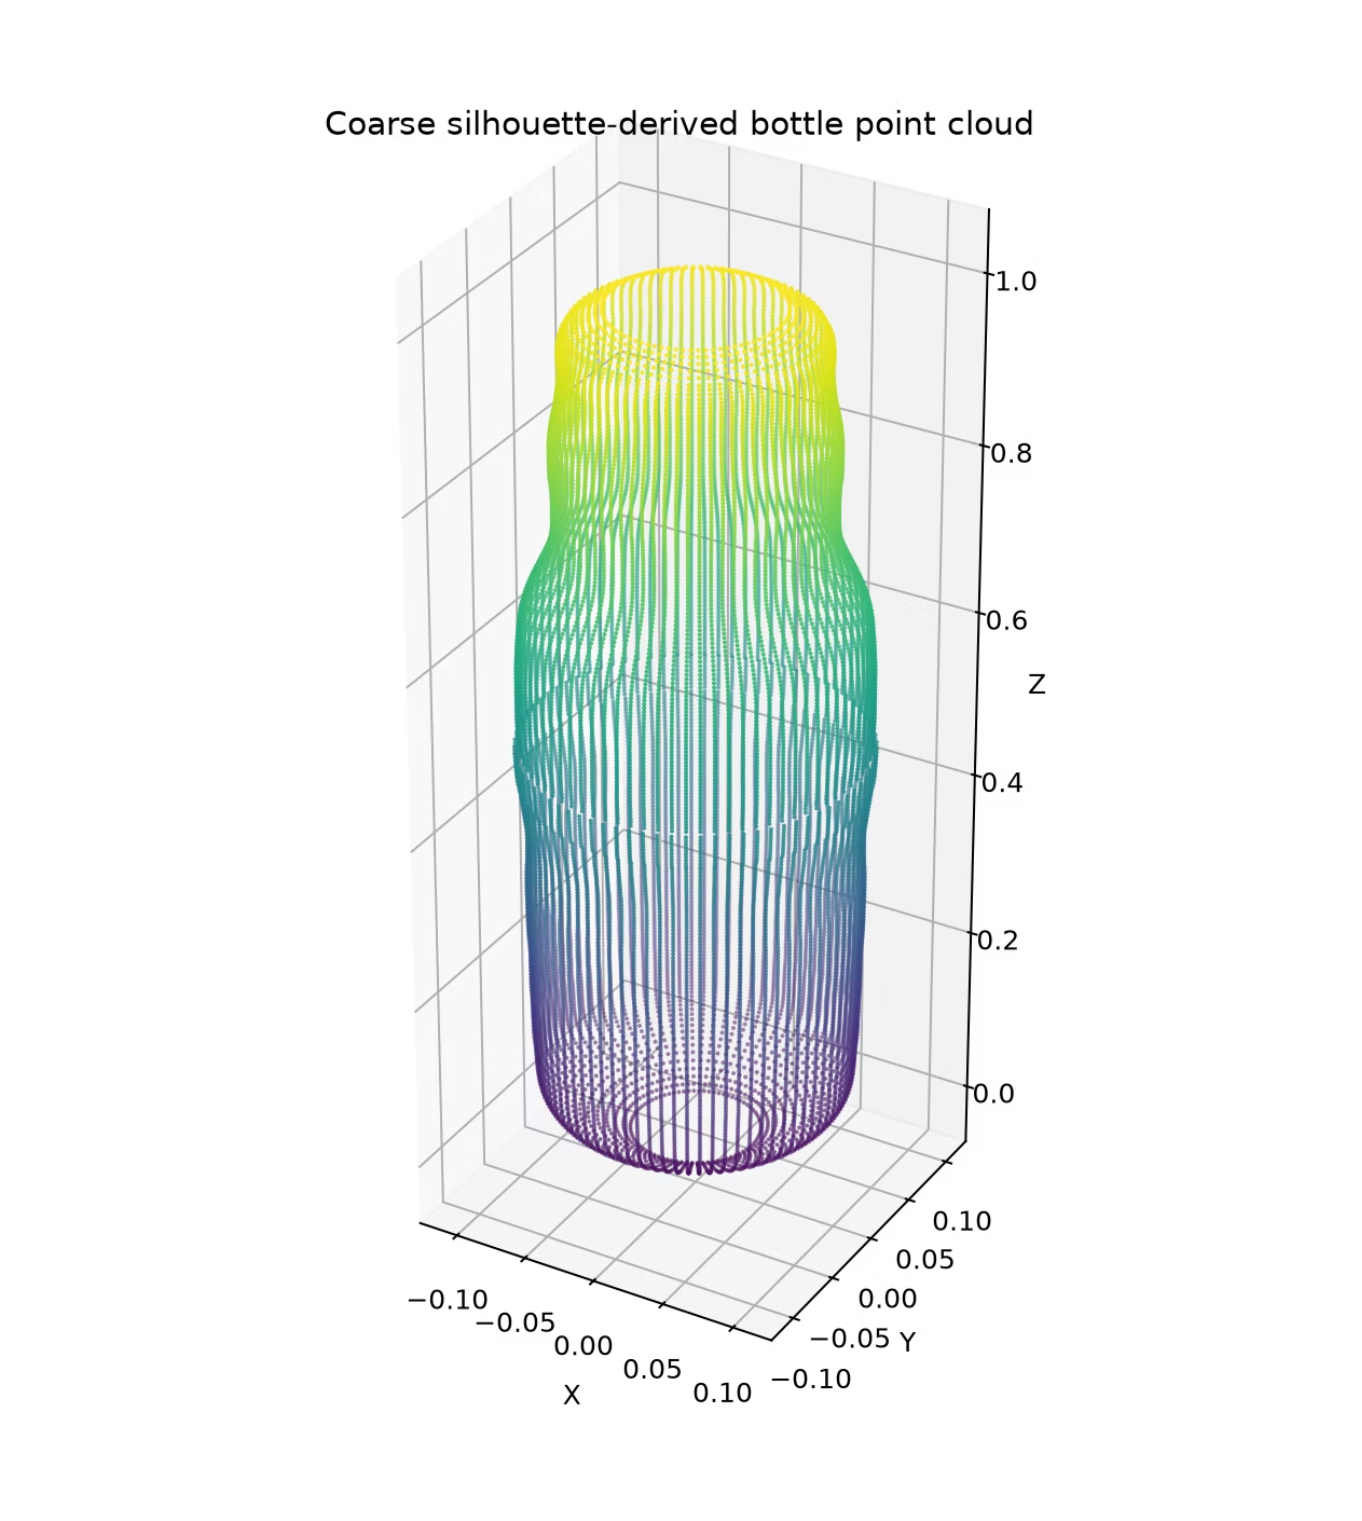
\includegraphics[width=0.95\textwidth,height=7.0cm,keepaspectratio]{figures/bottle.png}
\caption{Bottle prototype visual supplied in the progress presentation. Geometry is silhouette-derived with rotational symmetry.}\label{fig:bottle}
\end{figure}
\FloatBarrier

\subsection{Watch and Remote Results}
The watch experiment records 64,511 object points and 90,000 background points. The remote records 80,258 object points and 90,000 background points. The logs report successful point-cloud generation and, for the watch, read-back verification of points, colors, and normals. Figures~\ref{fig:watch} and~\ref{fig:remote} reproduce the corresponding supplied presentation visuals.
\begin{figure}[htbp]\centering
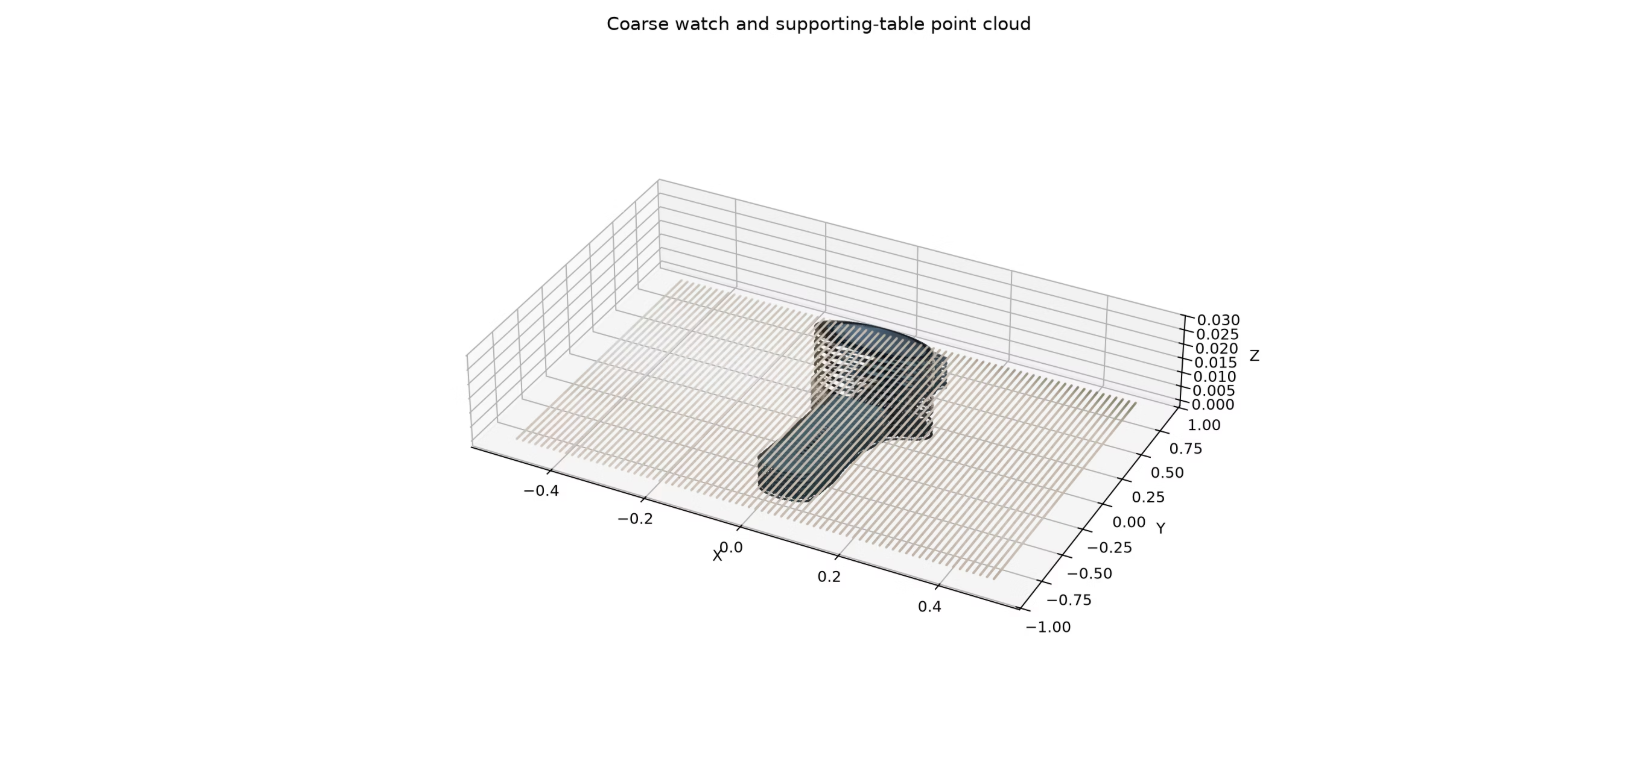
\includegraphics[width=0.95\textwidth,height=6.0cm,keepaspectratio]{figures/watch.png}
\caption{Watch prototype visual from the progress presentation. Case and strap heights are assigned; the table and unseen underside are planar.}\label{fig:watch}
\end{figure}
\begin{figure}[htbp]\centering
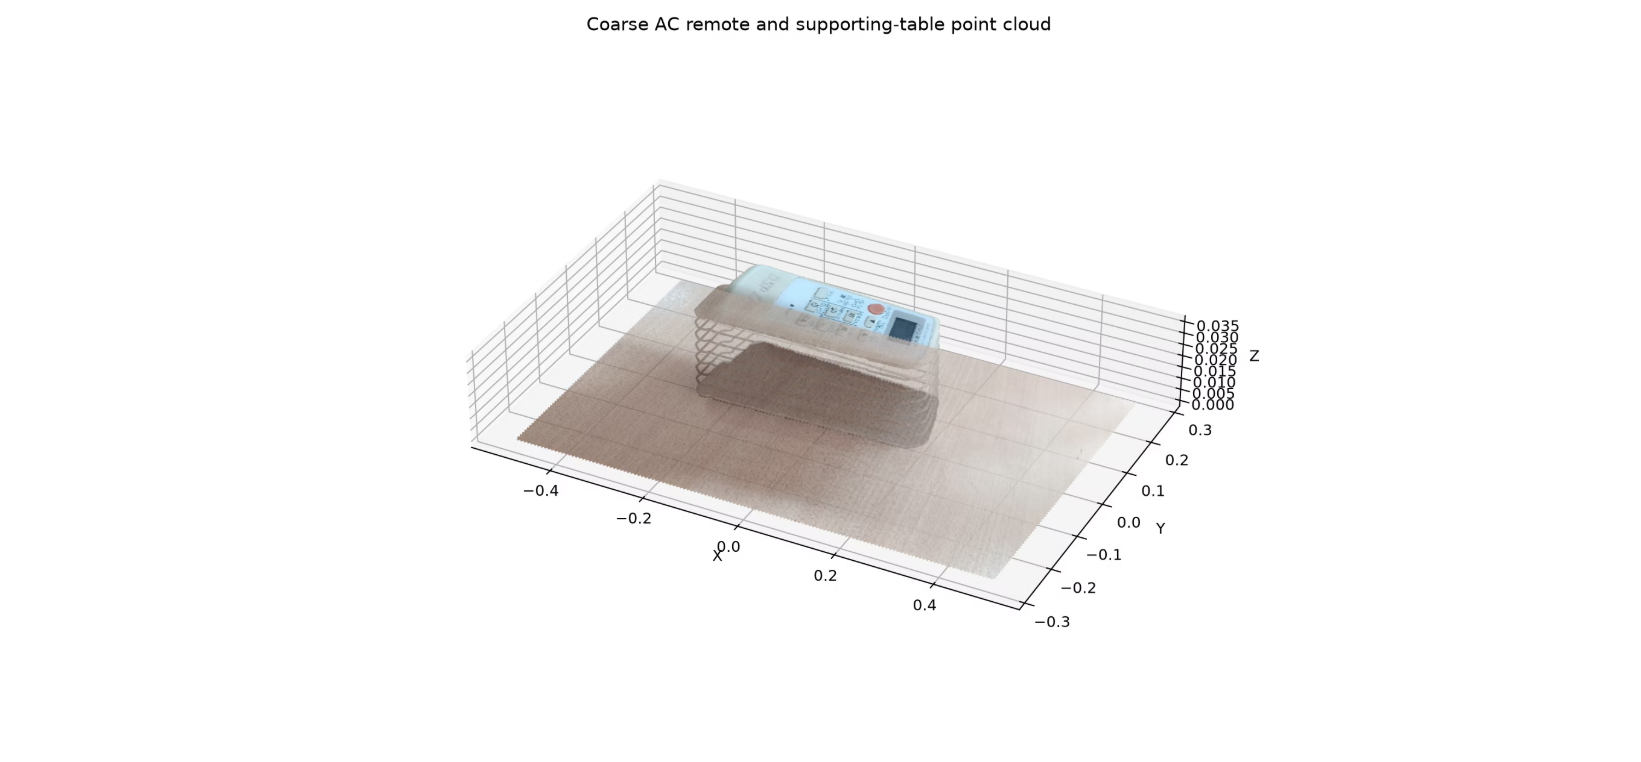
\includegraphics[width=0.95\textwidth,height=6.0cm,keepaspectratio]{figures/remote.png}
\caption{AC remote prototype visual from the progress presentation. The single-view model uses an assumed object height and planar background.}\label{fig:remote}
\end{figure}
\FloatBarrier

\section{Analysis and Discussion}
The three experiments demonstrate the practical steps needed to transform a foreground mask into a colored point cloud and inspect the exported result. They also reveal different segmentation failure modes. The bottle can be outlined by a pretrained model despite semantic ambiguity. The watch requires a scene-specific color-based fallback. The remote uses an initialized foreground/background segmentation procedure. These choices show that reliable object boundaries require explicit evaluation before stereo integration.

The prototypes do not solve the project's central occlusion problem. Bottle symmetry constructs unobserved surfaces; watch and remote extrusion assign depth; background completion copies texture into a region that was hidden. None of these operations estimates a moving object's historical geometry from calibrated stereo observations. Their contribution is an initial workflow and a set of concrete limitations that guide the next experiments.

Point count cannot substitute for fidelity. Counts depend on sampling parameters, and the watch and remote totals include 90,000 background samples each. Without a reference surface and a fixed sampling protocol, a denser cloud may have no greater geometric accuracy. Similarly, successful file read-back confirms output integrity but does not validate surface shape or scale.

\section{Progress Against the Planned System}
The presentation identifies five stages. Initial object reconstruction prototypes are complete. Object identification and edge handling are ongoing, with inference tried and systematic boundary evaluation pending. The stereo depth foundation is ongoing at the preparation/integration stage; no calibrated depth result is reported. Partial-occlusion handling and temporal reconstruction are planned.

There are no reported stereo depth errors, geometric F-scores, temporal stability measurements, recovery times, or per-frame runtime results in the current evidence. Consequently, this report does not claim a quantitative improvement over a stereo baseline or a real-time occlusion-recovery demonstration. These measurements are required before the proposed method can be judged against its objectives.

\section{Limitations and Threats to Validity}
The current inputs are few and object-specific. Bottle capture quality limits correspondence evidence, while the watch and remote use only one view for their coarse model. Chosen heights, arbitrary scale, symmetry, planar completions, and copied texture restrict geometric interpretation. The prototype techniques also differ, so their counts are descriptive rather than comparative results.

For future evaluation, calibration error, imperfect synchronization, segmentation bias, and motion-estimation failure may interact with occlusion handling. Tuning and reporting on the same sequences would overstate performance. The planned matched conditions, held-out tests, component ablations, and separate accuracy/coverage metrics are intended to expose those effects. They have not yet been executed.
